\documentclass[a4paper,12pt]{report} % report, 12pt
\usepackage[utf8]{inputenc} % utf8
\usepackage{graphicx} % images
%\usepackage[pdf]{pstricks} %compilation pdf graphics
\usepackage[english]{babel}
\usepackage[T1]{fontenc} % accents

\usepackage{fancyhdr} %en-têtes et bas de page
\pagestyle{fancy}
\setlength{\headheight}{15pt}
\setlength{\footskip}{60pt} 

\usepackage{times} % Times New Roman

\usepackage{titlepic} %picture page garde

%%\usepackage{hyperref}% pour le \url

\title{Team Work Report in \LaTeX}
\titlepic{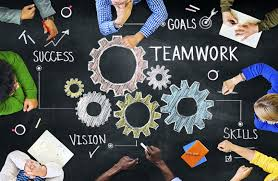
\includegraphics[width=0.7\textwidth]{teamwork.jpeg}}	 
\author{Grégoire MEUNIER}
\date{Date of writing : \today}

%Definition des en-têtes
\fancyhead[L]{Grégoire Meunier}
\fancyhead[C]{\today}
\fancyhead[R]{Team Work Report}	

\fancyfoot[C]{\thepage}
\fancyfoot[R]{
\includegraphics[scale=0.2]{logo_utc.png}}
\fancyfoot[L]{
\includegraphics[scale=0.15]{logo_tuke.png}}

\renewcommand{\contentsname}{Contents Table}




%-----------------------------------------------------------------------------------BEGIN DOCUMENT---------------------------------%
\begin{document}
% --------------------------------------------------------------------PAGE DE GARDE------------------------------------------------%
\maketitle
% --------------------------------------------------------------------SOMMAIRE-----------------------------------------------------%
\tableofcontents

%--------------------------------------------------------FIRST CHAPTER-------------------------------------------------------------%
\chapter{What is Conflict Management ?} \newpage
Your goal is to makes the conflict happens the better you can. The final result of that conflict should be that every part of the conflict had clearly discribed what they wanted. Then we arrived in the situation that everyone’s wants and needs were respect during the process of resolution.\footnote{We used this article \cite{Cmana:1} for this chapter.}
%------------------------------------------FIRST SECTION---------------------------------------------------------------------------%
\section{Different type of conflict management}
\subsection{Preventative measures}
It takes time to use this way, but it sure will be efficient.
\begin{itemize}
\item Workplace changes : Reorganise the framwork of the place.
\item Training staff : Know exactly what everybody has to do.
\item Conflict resolution policy : Give to your people access to training in communication.
\end{itemize}
\subsection{Alternative dispute resolution}
When basique methods doesn't get success, we need to go deeper in the problem. Make people talk with differents people in the way to find an arrangement.
\begin{itemize}
\item Informal discussions : Make people in the conflict talk together while you stay impartial. It gives people time to understand each other and to start again on a good basement.
\item Mediation : A third person that make people talk in a good environment in the way to solve problems. People calm down and find a good conclusion to fix the situation.
\item Conciliation : A third person who makes people talk and decide for them what they shloud do in order to fix the solution.
\item Arbitration : It is more official than previous methods. There is lawyers defending each person and an arbitrator to impose a legally-blinding settlement.
\end{itemize}
%----------------------------------------SECOND SECTION----------------------------------------------------------------------------%
\section{Causes of conflict at Work}
First of all, it is mostly because of several persons, and not because of just one of them. The goal here is to understand clearly what is the problem and act positively in order to prevent it from happening another time.
\subsection{Common causes of conflict at work}
\begin{itemize}
\item Differences in personality : Understand others cultures and backgrounds is primordial in a teamwork, everybody doesn't have the same character.
\item Differences in styles of working : Everybody has his own speed of working, you should not impose your speed to others.
\item Miscommunication or misunderstandings : Take care of what has understand everybody.
\item Availability of ressources : Asking could be very difficult for some people, so take care of providing everything your people needs.
\item Level of support : Some people need to be supported. If they do not feel a person behind us who his encouraging them, they will feel alone and do a bad work.
\item Poor customer service : Understand what the client wants is very important to understand what is our work.
\item Poorly-organised workplace : Have a good framework, place to realx, to be alone, to rest a while permit to people to be more efficient at work.
\item Poor management : Take care to have a strong person leading the team. Without this person, the team feels weak and loose confidence and motivation in the work.
\item Discrimination, harassment, etc. : Some kind of pratics are illegals. You should avoid that sort of problems from your team. If you don't stop before it starts, it gonna takes you time, money and power. And moreover, it gonna give a bad vision of your company.
\item Contract of employment : You should take care of what people have to do and try to spare the "bad" stuff and do not give it to the same person. If you do, that person will feel angry and put a bad ambiance in your team.
\end{itemize}
%---------------------------------------THIRD SECTION-----------------------------------------------------------------------------%
\section{Top Tips for Managing Conflict in the Workplace}
After having enumerate all the problems you can have at work, I gonna write here some examples to follow before having any troubles.
\begin{enumerate}
\item \textbf{Do a conflict risk assessment :} Check the relations between member of your team in order to see conflict coming.
\item \textbf{Don’t ignore it :} If their is a problem, do not forget it. You should solve the situation before it gets worse.
\item \textbf{Put in place an ‘open door’ policy :} Be open-minded and take in consideration what your employees are telling you. Do not hesitate to remind to your people that you are here if there is any problem.
\item \textbf{Promote differences :} Show to your team that people with a singular way of doing are still accepting in your team if it is effective. Remember a team is made of individual : different skills, different abilities.
\item \textbf{Become a mediator :} You should be or have a person in charge of people that be able to make people talk together and who is capable to put on the table a acceptable solution for each part of the conflict.
\item \textbf{Set clears goals and expectations :} You should frame everything in order that your team can understand clearly their missions.
\item \textbf{Give and seek regular feedback from your team :} Learn to lissen actively your team and do not hesitate to go to them in the way to get their opinion.
\item \textbf{Stay calm and in control :} Do not forget that the role model behaviour and value : do what I do not what I say.
\item \textbf{Attack the problem, not the person :} Accept the difference is your team. Attack the person won't change her but only give her the opportunity to become agressive.
\item \textbf{Be positive, focus on positivity :} If you stay positive even in bad situations, your people gonna do the same. Another time, give them the right exemple to follow.
\end{enumerate}

%--------------------------------------------------------SECOND CHAPTER------------------------------------------------------------%
\chapter{Difference Between Group and Team}\newpage
When two or more individuals are classed together either by the organization or out of social needs, it is known as a group.
On the other hand, a team is the collection of people, who are linked together to achieve a common objective.
When we talk about groups and teams we use the terms interchangeably – it is possible to have a group without a team but not a team without a group. 
\footnote{We used this article \cite{GroupTeam:2} and this other one \cite{GroupTeam:3} for this chapter.}
%-------------------------------------------FIRST SECTION-------------------------------------------------------------------------%
\section{Definition of Group}
The word group however has a broader meaning – a group of passengers on a flight have a common characteristic – to travel, but they are not necessarily working towards a common cause. Groups do not even need to refer to people, for example, a group of products in a supermarket, in this case the group is arbitrary and could be defined by any number of variables.
\subsection{Important Defining Features of Groups:}
\begin{itemize}
\item People who can identify with each other.  Sharing ideas, beliefs and/or experience of common areas.
\item People who frequently and regularly engage with each other, agreeing on a purpose and working together on shared tasks.
\item People who recognise themselves and are recognised by others as part of a group.
\end{itemize}
\subsection{Why Form Groups ?}
Managers recognized many years ago that two heads are better than one, thus small businesses have turned to groups or departments for many reasons. With group work, members have a shared knowledge of the group’s objectives, but specific tasks or responsibilities are assigned to different individuals. By separating work into groups – such as one devoted to marketing, one devoted to accounting, etc. – individuals within those groups are able to maximize their expertise on a long-term basis.
%------------------------------------------SECOND SECTION-------------------------------------------------------------------------%
\section{Definition of Team}
A team is generally more specific.  We would not refer to our airline passengers as a team, unless they crashed on a desert island and needed to work together to survive.  The distinction is that a team is working together for a common cause. A group of schoolchildren may be in the same class, whereas a team of schoolchildren may be working together on a specific project within the class.
% \begin{enumerate}
% \item 
% \end{enumerate}
\subsection{Why Form Teams ?}
Businesses form teams usually to tackle a specific – and usually temporary – goal or project with the intent of leveraging the collective expertise of a variety of people. Because experts from various departments are involved, teams can avoid potential problems early on in a project. For instance, a team of only engineers may create a new product but may not understand whether it’s affordable until someone with a finance background completes a “return on investment” or ROI analysis on its feasibility. Having a finance member involved in the team from the beginning will help the engineers to create an affordable product in the first place, saving time and resources. Teams can be very productive because involving people with different talents provides teams with increased opportunities to work more efficiently.
%------------------------------------------THIRD SECTION--------------------------------------------------------------------------%
\section{Comparison}
\begin{table}[h]
\begin{center}
\begin{tabular}{|c|c|c|}
\hline
Basic For Comparison & Group & Team\\
\hline \hline
Members & Independant & Interdependant\\
\hline
Work Products & Individual & Collective\\ \hline
Leadership & Only one leader & More than one\\
\hline
\end{tabular}
\end{center}
\caption{Comparison Chart}
\label{Comparison Chart}
\end{table}

%--------------------------------------------------------THIRD CHAPTER------------------------------------------------------------%
\chapter{Managing a team/project}\newpage

The management team is the group of individuals that operate at the higher levels of an organisation and have day-to-day responsibility for managing other individuals and maintaining responsibility for key business functions. \newline
The management team is also generally responsible for putting together the business strategy and ensuring the business objectives are met. The Management team are held accountable by the companies board of directors. \newline
Some organisations may operate a fairly flat team hierarchy with one or just a few layers of management while other companies may operate with several layers of the management team.
\footnote{We used this article \cite{Manager:4}, that one \cite{Manager:5} and this other one \cite{Manager:6} for this chapter.}

%-------------------------------------------FIRST SECTION-------------------------------------------------------------------------%
\section{Exemple of managing a team/project}
Here, I am giving you an example of what could be the perfect way to work as a team. This example was made by myself and it give you a subjective you of a good team. \newline \newline
\textbf{Goal :} Create something eco-friendly in the way to make people gain interest in global ecology \newline
\textbf{Team :} Fifteen (15) people are currently working on that project with me and I manage several departments where the fifteen people are working inside \newline
\textbf{Departments :}
\begin{itemize}
\item Thinking about the product and improving it continuously : \textit{5 people}
\item Calculate the cost and everything about the viability of the product : \textit{2 people}
\item Making the board of what has to be done (ask team 1) : \textit{3 people}
\item Making the product, the communication about it and tell team 1 what has to be improved : \textit{5 people}
\end{itemize}
\textbf{My duty :} I have to check that every process of the project is working well and each person has really understand what we have to do. \newline
\textbf{Final situation :} The team is working well and the product is always improving it-self thanks to the teams who checks at every time of the production --> there is not an external team in charge of the checking process but everybody is doing it because everyone could have a good proposition. \newline
%------------------------------------------SECOND SECTION-------------------------------------------------------------------------%
\section{Be a good manager}
Learning how to be a good manager is a combination of effort, understanding your role as a manager, your team’s role as your employees, and a bit of practice. Whether you were just promoted to your first managerial role or if you are simply looking for ways to become a better manager, you should follow thoses simply rules.
\subsection{Tips on How to Be a Good Manager: New Managers}
\begin{itemize}
\item Strengthen Your Own Skills
\item Lead By Example
\item Ask for Feedback from Other Managers or Executives
\item Set Achievable Goals for Yourself and Your Team
\item Use Your Time Wisely
\item Be Consistent
\item Understand Your New Relationships with Former Peers
\end{itemize}
\subsection{Key Questions for Experienced Managers}
\begin{itemize}
\item Am I still leading by example ?
\item Am I still current with my skills ?
\item Have I asked for feedback lately ?
\item Am I setting achievable metrics and goals ?
\item How is my time management ?
\item Am I consistent ?
\item Have I created good relationships with my team members ?
\end{itemize}
\subsection{Tips for How to Get Back to Being a Good Manager}
\begin{itemize}
\item Get Back Into “The Trenches”
\item Try a Survey For Honest Feedback from Team
\item Hone Your Managerial Skill Set
\end{itemize}
%------------------------------------------THIRD SECTION--------------------------------------------------------------------------%
\section{Managing in France and in Slovakia}

\includegraphics[scale=0.30]{france.jpg}
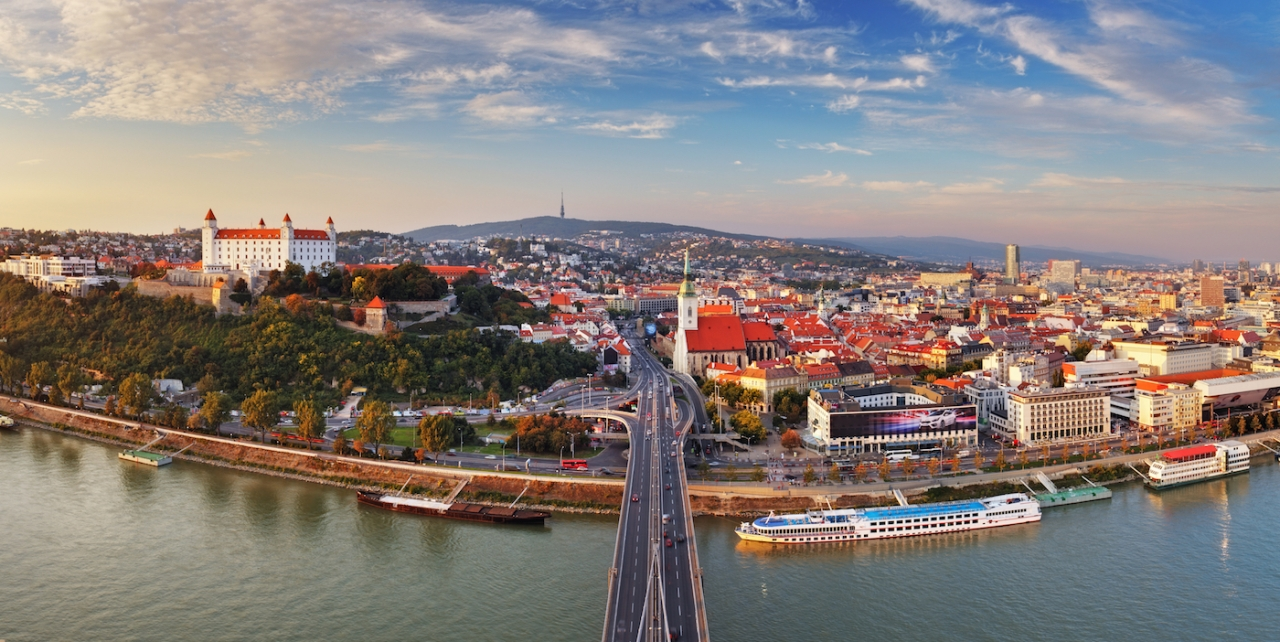
\includegraphics[scale=0.45]{slovakia.jpg}
\newpage
\subsection{Slovakia part}
The Slovak Republic also enjoys a well educated, skilled and cheap labour force, a flat rate of taxation for corporations and individuals, no dividends taxes, liberal labour laws and a favourable geographical location, compared to Western Europe. This has helped to increase foreign direct investment by about 600\% in the last 10 years.
Slovak attitudes to foreigners in business are that of mutual respect. They respond well to foreigners when they see that they can learn from them, but can be intolerant of those who do not appear to deserve their position. The days of blind adulation for everything foreign are long gone. Slovaks have utmost respect for expatriates working in the Slovak Republic, but now that respect is more for the knowledge of the individual rather than just because they are foreign.
\subsection{France part}
Management in France, we learned, is considered a “state of mind” rather than a set of techniques. According to executives like Michel Lafforgue, directeur général technique at L’Oréal, the successful development of executives depends on creating a distinctive shared identity, a sense of belonging to the French managerial class.
France has come closer than any other nation to turning management into a separate profession, with its own entry requirements and regulations. Managerial status in France is not part of a graded continuum, but rather a quantum leap, involving a change of legal status (for example, in terms of pension entitlement) as well as subtle changes in outlook and self-perception.
A massive survey of foreigners working in France has revealed that the French management style is far from being an international role model - but the extended lunch breaks, at least, were a redeeming feature. We take a closer look at the findings.

% \footnote{Texte de la note.}

%------------------------------------------------------------------------BIBLIOGRAPHIE--------------------------------------------%
\bibliographystyle{plain}
\bibliography{bibli.bib}


\end{document}

